\documentclass[11pt,a4paper]{article}

\usepackage{geometry}
 \geometry{
 a4paper,
 total={150mm,237mm},
 left=30mm,
 top=30mm,
 }

% cf. http://tex.stackexchange.com/questions/50182/subtitle-with-the-maketitle-page
\usepackage{titling}
\newcommand{\subtitle}[1]{%
  \posttitle{%
    \par\end{center}
    \begin{center}\large\textbf{#1}\end{center}
    \vskip0.5em}%
}

\usepackage{color}
\usepackage{graphicx}

\usepackage[utf8]{inputenc}
\usepackage[lf]{venturis} %% lf option gives lining figures as default; 
\usepackage[T1]{fontenc}
\usepackage{csquotes}
\usepackage[UKenglish,german]{babel}

\usepackage{fancyvrb}

\widowpenalty10000  % http://tex.stackexchange.com/questions/4152/how-do-i-prevent-widow-orphan-lines
\clubpenalty10000

\title{The SysSon Platform}
\subtitle{Technical Report TR-2016-08-1\\Institute of Electronic Music and Acoustics, Graz}
\author{Hanns Holger Rutz}
% \date{09-Feb-2016}
\date{August 2016}

% cf. https://tex.stackexchange.com/questions/94126/change-font-to-only-section-and-subsection-of-my-document
%\usepackage{titlesec}
%\titleformat{\chapter}[display]
%  {\fontfamily{pag}\selectfont\huge\bfseries}
%  {\chaptertitlename\ \thechapter}
%  {20pt}
%  {\Huge}
%\titleformat{\section}
%  {\fontfamily{pag}\selectfont\bfseries\Large}
%  {\thesection}
%  {1em}
%  {}
%\titleformat{\subsection}
%  {\fontfamily{pag}\selectfont\bfseries\Large}
%  {\thesection}
%  {1em}
%  {}

\usepackage[backend=biber,authordate]{biblatex-chicago} % citereset=chapter
%\usepackage[backend=biber,natbib,isbn=false,useprefix=true,sorting=ydnt]{biblatex-chicago} % citereset=chapter
\addbibresource{all.bib} % add a bib-reference file
\addbibresource{rutz.bib} % add a bib-reference file

% warning: https://tex.stackexchange.com/questions/313477/
% \usepackage{csquotes}

\usepackage{tabularx}
% cf. https://tex.stackexchange.com/questions/84400/table-layout-with-tabularx-column-widths-502525
\newcolumntype{s}{>{\hsize=1cm}X}

% says you should load after babel and fontspec
\usepackage[shrink=10, babel=true]{microtype}	% http://tex.stackexchange.com/questions/141852/latex-allows-line-break-between-concluding-em-dash-and-comma-before-a-new-sub-cl/141854#141854

% has to come first for full scale TeX voodoo bullcrap
\usepackage{hyperref}
% get rid of the horrible coloured boxes around links
\hypersetup{
    colorlinks,%
    citecolor=black,%
    filecolor=black,%
    linkcolor=black,%
    urlcolor=black
}
% has to come after frickin hyperref
\VerbatimFootnotes

\newcommand{\todo}[1]{\colorbox{yellow}{\textsc{todo}: #1}}

\newcommand{\quot}[1]{\guillemotleft {#1}\guillemotright}

\newcommand{\worktitle}[1]{\textit{#1}}

\newcommand{\workentry}[2]{\vspace{7.5pt}\noindent\textbf{#1} (#2)}
\newcommand{\workentrySel}[2]{\vspace{7.5pt}\noindent\textbf{#1}$*$ (#2)}

\newcommand{\figref}[1]{Fig.~\ref{#1}}

\newcommand{\software}[1]{\textit{#1}}

\newcommand{\sysson}[0]{SysSon}
\newcommand{\syssonVersion}[0]{1.8.0}
\newcommand{\syssonVersionS}[0]{1.8.0-SNAPSHOT}

\newcommand{\artefacts}[0]{\textsc{Artefacts:}}
\newcommand{\assessment}[0]{\textsc{Assessment:}}

\begin{document}
% \begin{titlepage}
\maketitle
\selectlanguage{UKenglish}
\thispagestyle{empty}
\newpage
\section{Statement}

The next sub-sections lists the main points of the WTZ project, followed by an outline for the preparation of the first milestone.

\subsection{General Mission Statement}

\begin{itemize}
\item to understand the specific expertise of artists and the potentials of transfer of knowledge from research in the arts into applied contexts
\item to define the interfaces necessary to warrant a successful application of approaches and prototypes that have been developed in long-term practice
\item conduct a series of self-standing case studies, generate best practices examples
\item interdisciplinary process of artistic research and natural sciences and engineering: assess and document
\item production of a catalogue of criteria for future reference
 translation of artistic research ``results'' from proof-of-concept status to a status with greater number of recipients and users.
\end{itemize}

\subsection{Project Year 1 -- SysSon}

\begin{itemize}
\item a case study is developed based on the prototype of a sonification software
\item collaboration between IEM and WegC
\item WegC staff is user group along with which prototype is elaborated, creating a product usable in their work
\item development of sonification templates; creation of a suitable platform, distribution and integration
\item systematic documentation; basis for successive project year
\end{itemize}

\section{Areas for Development}

\subsection{Sonification Design}

\begin{itemize}
\item Seamless transitions between server and client side processing
\item Modularity of sounding components
\item Better programmatic access to matrices
\item Pre-processing stages for matrices
\item UI: programmatic building blocks for control elements
\end{itemize}

\subsection{Sonification Usage}

\begin{itemize}
\item Integration: IPython / Jupyter, etc.; Scala in ``Data Science''
\item Stronger linkage between sounding and visual components
\item Wizards, guided building blocks
\item Import/export interfacing
\item UI: docking framework, usability
\item Specific scenarios, e.g. presentation tool for a conference, export for a web-site
\end{itemize}

\subsection{Overall Computer Music Perspective}

\begin{itemize}
\item UI: Linkage between text editing and visual components
\item ``Thinking tool''; note-pad, mark-down, hyper-text, mind-maps, small-talk
\end{itemize}

\section{Next Planning Stage}

In the meeting of 12-Aug-2016, it was decided that the strategy will focus on the development of the sonification templates, in iteration with select individuals from WegC over a longer period. Development of the software must be carefully planned in order to produce achievable milestones with the available resources. As a first step, the work effort for implementing the following changes should be assessed:
%
\begin{itemize}
\item Improving the sonification editor user interface by adding a few widgets such as buttons, toggle switches etc., being able to control their layout broadly.
\item In conjunction, being able to branch in the synth graph, i.e. being able to select different sub-programs based for example on the user interface elements.
\item Possibility of subjecting these branches to real-time interactive control (vs. simply evaluating at the beginning of the play action)
\end{itemize}

\subsection{Sonification UI Elements}

The current code for determining control elements is in \verb!SonificationViewImpl! method \verb!updateGraph!, with the following scanning process:
%
\begin{verbatim}
val userValues  = g.sources.collect { case graph.UserValue(key, default) =>
  val cell = CellView.exprMap[S, String, Double, DoubleObj](controls, key)
  val view = DoubleSpinnerView.optional[S](cell, name = key.capitalize, 
    default = Some(default))
  (key, view)
}
\end{verbatim}
%
In other words, we require that \verb!UserValue! elements are found on the top level, and in the order of their appearance we build double-spinner-views. The idea is shown in \figref{fig:ui}

\begin{figure}%
\centering%
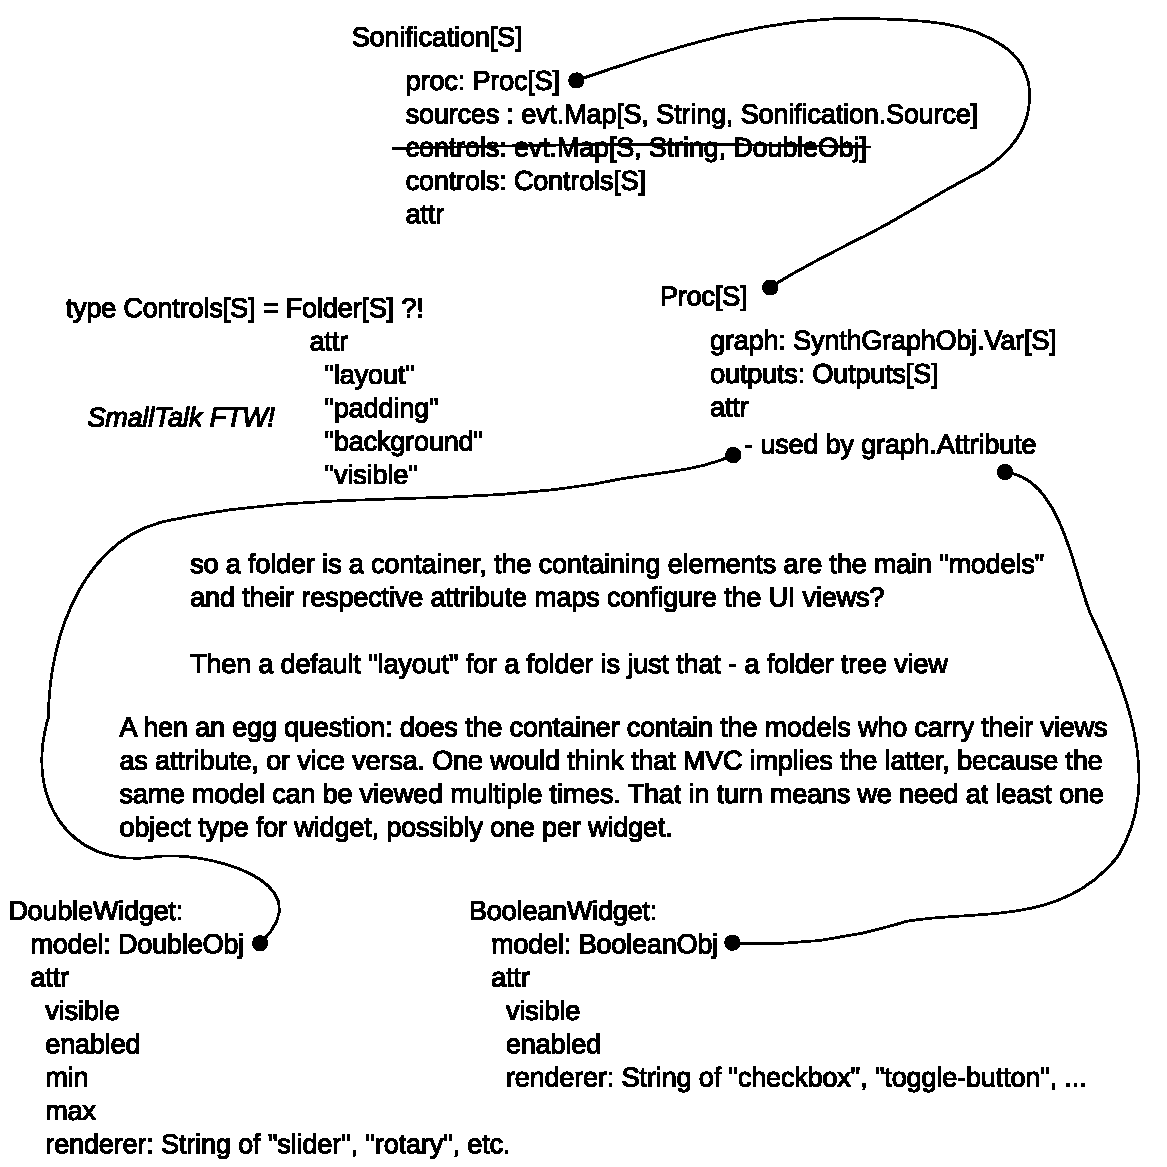
\includegraphics[width=0.8\textwidth]{figures/discuss_ui.pdf}%
\caption{Concept for simple UI definitions.}%
\label{fig:ui}%
\end{figure}

\subsubsection*{Discussion}

User values are then stored in the \verb!controls! field of the sonification object, a map from control names to double objects. If we ensure that an \verb!S#Var! is always used here, we can uses that as a reference for further UI coding. Let's assume we had the possibility to create an expression for an option of a map entry, like \verb!controls.getRef(key): DoubleOption!. Then we could somehow boil that down to a flat expression, like \verb!.getOrElse(DoubleObj.Const(0)): DoubleObj!.\footnote{Another possibility is to have \verb!controls.getOrElseRef(...): DoubleObj! and avoid having to introduce the option object, which is probably a good ideas as we still have no support for objects with type-parameters and would have to define an option object for any peer type.} Then we can transform it into a boolean, like \verb!.>(thresh): BooleanObj! and store it inside a user interface element attribute such as \verb!visible! or \verb!enabled!.

Then the next question would be how we can define those expressions and expression-combinators from within \software{Mellite}? This looks like a bit more work. Perhaps the best option here is to have built-in context menu functions to produce the most common expressions.

Now if we have a simple additional UI editor anyway---because we want to be able to style the elements slightly, position them etc.---then it would make sense to remove \verb!graph.UserValue! and simply use the existing \verb!graph.Attribute!. And then indeed we should introduce a \software{ScalaCollider}-like \verb!"key".kr! shortcut. The sonification editor could still listen to graph updates and ``notify'' the developer about newly appearing attributes, offering to create UI elements for them. We could repurpose \verb!.controls! so that we rely on the double-object's attribute map to store the type of widget and widget parameters, adopting \verb!ParamSpec! from \software{Wolkenpumpe}, etc. We wouldn't even need the \verb!.getRef! because now we could refer to the \verb!S#Var! directly.

Since this principle is general, it should be decomposable into things directly within \software{SoundProcesses}. For example, we could even completely diminish \verb!.controls! if attributes are stored with the \verb!Proc!'s attribute map. Instead we would just associated a simple \verb!Panel! object. It makes sense to start a new sub-module within the \software{Lucre-Swing} project.

\subsection{Conditional Synth Sub-Graphs}

This is a quite complex issue, as it touches the internals of \software{SoundProcesses} (how and when to build synth graphs, how they access the outside context, etc.) and the serialisation of synth graphs. One has to distinguish two cases
%
\begin{itemize}
\item determination at initialisation time \emph{on the client side}
\item determination \emph{on the server side} (the distinction between scalar rate or initialisation time and audio rate is less relevant)
\end{itemize}
%
It also affects the question whether a sound model should be described by one monolithic synth graph or rather by a connected collection of graphs.

\subsubsection*{Discussion}

Let us first explore the case where branching is solely solved \textbf{inside one monolithic synth graph function.} There are two possibilities: Stick to the \verb!GE! (graph elements) ``interpreter'' approach, where a \verb!SynthGraph! is directly serialised. This is the more ``functional'' style. Or allow instead to execute a \verb!Function0[SynthGraph]!, similar to the \verb!Action! object, and going for a more ``imperative'' style.

\textbf{In the functional style,}\footnote{This becomes a sort of proof for ``Greenspun's tenth rule'': \url{https://en.wikipedia.org/wiki/Greenspun's_tenth_rule}} we would have a restricted set of pseudo-UGens or graph elements that handle the branching. For client-side initialisation time, we might have something like
%
\begin{verbatim}
// possibly: IfAttrGt.ir
val amp: GE = ???
val res: GE = IfAttrGt("key", 0) {
  WhiteNoise.ar(amp)
} ElseIfGt(1) {
  SinOsc.ar(441) * amp
} Else {
  DC.ar(0)
}
\end{verbatim}
%
The disadvantages here are that
\begin{itemize}
\item we might need a large number of graph elements for the possible comparison cases, \verb!IfAttr("boolean")!, \verb!IfAttrEquals("key", value)!, etc.
\item there is no possibility to perform general arithmetic operations on the attribute value. For example, if the attribute is a buffer, we might want to check the duration of the buffer. It does not make sense to define an entire new language interpreter here.
%\item We will most likely want to use graph elements from the outer context as input to the branches. The UGen graph builder thus must be capable to detect these dependencies and implicitly insert 
\end{itemize}
%
A potential advantage is that we could extend this syntax to theoretically support real-time branching:
%
\begin{verbatim}
val amp: GE = ???
val res: GE = IfAttrGt.kr("key", 0) {
  WhiteNoise.ar(amp)
} ElseIfGt(1) {
  SinOsc.ar(441) * amp
} Else {
  DC.ar(0)
}
\end{verbatim}
%
However, this produces two difficult implementation problems:
%
\begin{itemize}
\item We need to capture the dependency of the inner branches on the outer context, i.e. here the use of the signal \verb!amp! that must---upon expansion---be modelled by a bus between two synths, where the branches are conditionally created synths.
\item We need to capture the dependency of the outer context on the result of the conditional, i.e. here the further use of the signal \verb!res! that again must be modelled by a bus between two synths.
\end{itemize}
%
If this implementation is solved, it will make this approach very powerful, though, and client vs. server solution could be transparently determined from pattern matching. E.g.
%
\begin{verbatim}
If ("key".ir > 0) { ... }
\end{verbatim}
%
This would capture a \verb!BinaryOpUGen! which could be analysed for its rate and operands, possibly erasing to a real boolean check on the client side if the rate is \verb!scalar!, one operand is an attribute and the other a constant. This way, still arbitrary arithmetic expressions can be used, although without the guarantee that they are indeed erased to a boolean type and so might end up creating a second (possibly paused) synth.

The pausing synth of course could cause other problems, but it might be a sensible approach, as the programmer can still explicitly go for entirely non-paused branches using standard UGen comparators such as \verb!sig_==! and multiplications with zero or one.

\textbf{In the imperative style}, instead of evaluating code that produces a \verb!SynthGraph! and serialising that graph, we serialise a function that when applied creates the \verb!SynthGraph!. This makes it possible to ask directly for the value of an attribute and branch based on it:
%
\begin{verbatim}
val amp: GE = ???
val keyVal: Double = "key".value
val res: GE = if (keyVal > 0) {
  WhiteNoise.ar(amp)
} else if (keyVal > 1) {
  SinOsc.ar(441) * amp
} else {
  DC.ar(0)
}
\end{verbatim}
%
This looks nice at the first look, but indeed is not that different from the \verb!If ("key".ir > 0) ...! variant that we sketched out before using UGens only. It is also clear that with this imperative example, we do not yet have a solution for real-time control of branches. In Scala, we also cannot enforce the side-effect freedom of the function, while the function might have to be evaluated multiple times, for example if we wish to scan the sources of the synth graph for matrix variables. We introduce two control exceptions now that have to be thrown if the context information is insufficient to build the graph; first within the function that builds the \verb!SynthGraph!, then in the UGen builder when the graph is expanded. In other words, this also introduces additional complexity, even before we evaluate the performance impact by having to go through one extra interpretation step. It would thus appear that the functional style variant is generally preferable, although we do not know yet whether an implementation is feasible.

Going away from a monolithic synth function, branches could also be represented by \textbf{multiple }\verb!Proc!\textbf{ or generally }\verb!Obj!\textbf{ instances}. For example, if one takes the \verb!Ensemble! type, there is a boolean expression that controls its playback. We would then relax the constraint that \verb!Sonification! wraps a single \verb!Proc! instance, instead allowing any type of \verb!Obj! to be used as peer, for example a \verb!Folder! or \verb!Ensemble!. The user interface could view models from not one but multiple objects, or models (attributes) could be shared among multiple objects. Then communication between branches must be explicitly established by the programmer, using regular \verb!Output! instances and connections. The aural views would automatically manage bus allocation as disabled (paused) objects would not produce a running synth (?). It feels almost like an \emph{orthogonal} approach to the monolithic one, in the sense that we could implement both independent of each other, as either might be better suited in a particular scenario. This multiple-objects approach certainly requires more work for the user interface, in order to make the management enjoyable without too much confusion. Additional problems might be the correct selection of attribute maps and the question of how running time information is provided for the objects that are facultatively added to the mix.

\subsubsection*{Summary}

I would therefore think that the strategy should be to start with the implementation of the \verb!If! graph element and then evaluate how far this gets us. There are most likely follow-up problem that must be addressed, such as the increased demand of inter-synth bus channels that asks for a smart bus-reuse in the topology, an endeavour currently not yet undertaken.

\section{Libraries and Modules}

This section serves as a status-quo document, detailing the current module structure of the software, with possible points of entry for further development and improvement.

\sysson{} is built with the \software{sbt} build tool.\footnote{\url{http://www.scala-sbt.org/}} \software{Sbt} manages module and library dependencies though a software called \software{Ivy} and using so-called \software{Maven} artefacts. Such artefacts are composed of a group-identifier, artefact-identifier, and a version string. For example, \sysson{} itself has group-id \verb!at.iem.sysson!, artefact-id \verb!sysson!, and current version \verb!1.8.0-SNAPSHOT!. The version scheme is the one proposed as \emph{Semantic Versioning}\footnote{\url{http://semver.org/}}, i.e. \verb!MAJOR.MINOR.PATCH!. The \verb!MAJOR! version indicates an entire new architecture, where the first stable generation is usually indicated by the digit \verb!1!. The \verb!MINOR! version indicates incremental changes, while the \verb!PATCH! version indicate bug fixes without change in functionality. In the Scala eco-system, the terminology is slightly different, where the major version is called "epoch", the minor version is called major version and the patch version is called minor version. So Scala 2.11.8, the latest release, has epoch 2, major version 11, and minor version 8 in the Scala terminology. We will henceforth use this naming scheme. The special suffix \verb!-SNAPSHOT! indicates that the version is not a stable released artefact but work in progress. Stable artefacts of libraries are published to a repository such a the public Maven Central,\footnote{\url{http://central.sonatype.org/}} and build tools can thus automatically download required artefacts based on a description of an application's dependencies.

The Maven based build tool \software{sbt} assumes a \emph{binary compatibility} between all minor versions, whereas the major version must be incremented when a binary incompatible change is introduced. A binary incompatibility means that the Java byte code of the library contains changes that make it unsafe for use with a caller that was compiled against a different version. This happens for example if a method has been removed from public API or changed in signature. Sbt automatically chooses the highest minor version if there are several transitive dependencies on the same artefact but with different minor versions, while it warns when transitive dependencies exist for the same artefact with different major versions. This also applies to the Scala version a library was compiled against, meaning that a binary file resulting from compilation against Scala 2.10.x (where x is any minor version) is binary incompatible with a binary file resulting from compilation against Scala 2.11.x (with 2.11.8 being the currently most recent release version). To ease this difficulty, sbt has introduced a mechanism called cross-versioning. Often Scala releases are still source compatible, and thus it is possible, for example, to compile the same source code against Scala 2.10.x and 2.11.x without changes. The artefacts will then be ``tagged'' by appending the major Scala version, e.g. the artifact-id becomes \verb!sysson_2.11! when compiling against Scala 2.11.x (this is independent of the regular Maven version).

This versioning scheme can be observed in the dependency graph that shows all the libraries and transitive libraries,\footnote{Transitive means a library A is used by another library B, and B is used by \sysson{}. Then A is a transitive dependency of \sysson{}.} generated by the \software{sbt-dependency-graph} plugin\footnote{The call is \verb!sbt dependencyDot!.} and shown in \figref{fig:dependencies}.\footnote{In the figure, lower level transitive third-party dependencies have been omitted for a clearer overview.} We can see the \sysson{} main artefact on the left-hand side with arrows pointing to immediate dependencies (libraries), which in turn point to other transitive libraries. Some libraries are published as a set of related artefacts, often bound together by one ``virtual'' meta-package. For example, the \software{Mellite} computer music environment is actually composed of two artefacts \verb!mellite-core! and \verb!mellite-views!, combined as virtual artefact \verb!mellite!. The \verb!-views! artefact connects to the graphical user interface, whereas \verb!-core! only contains data structures. Since \verb!-views! depends on \verb!-core! but not vice versa, it means we can develop a library merely based on the data structures without requiring the dependency on any GUI.

\subsection{Licensing Questions}

This approach helps keeping the code base modular, and furthermore can improve the licensing situation: In general we try to avoid dependency on GPL licensed code,\footnote{\url{https://www.gnu.org/licenses/gpl.html}} because it enforces the GPL on the entire product, something that is not the case with the LGPL\footnote{\url{https://www.gnu.org/copyleft/lesser.html}} or even more permissive licenses. We try to decouple GPL dependencies as far as possible, allowing for LGPL terms in most cases. GPL artefacts are often commercially developed products, because a commercial client company will likely not want to release their own product as open source under GPL terms and is thus forced to buy a commercial license from the library vendor, an approach that is called dual licensing. For example, the \software{iText} PDF library is available for free under GPL terms or by buying a commercial license that allows the client to develop their product without requiring to open source it. The same is true for the \software{Berkeley DB} database (developed by Oracle) and the \software{WebLaF} user interface look-and-feel. We currently do not own any commercially bought licenses, and thus \textbf{\sysson{} must be licensed under GPL version 3} terms. However except for the mentioned GPL based libraries, we have control over most other libraries, and thus in the future a different license might be chosen if replacements are found for the GPL libraries (or commercial licenses purchased).

\begin{figure}%
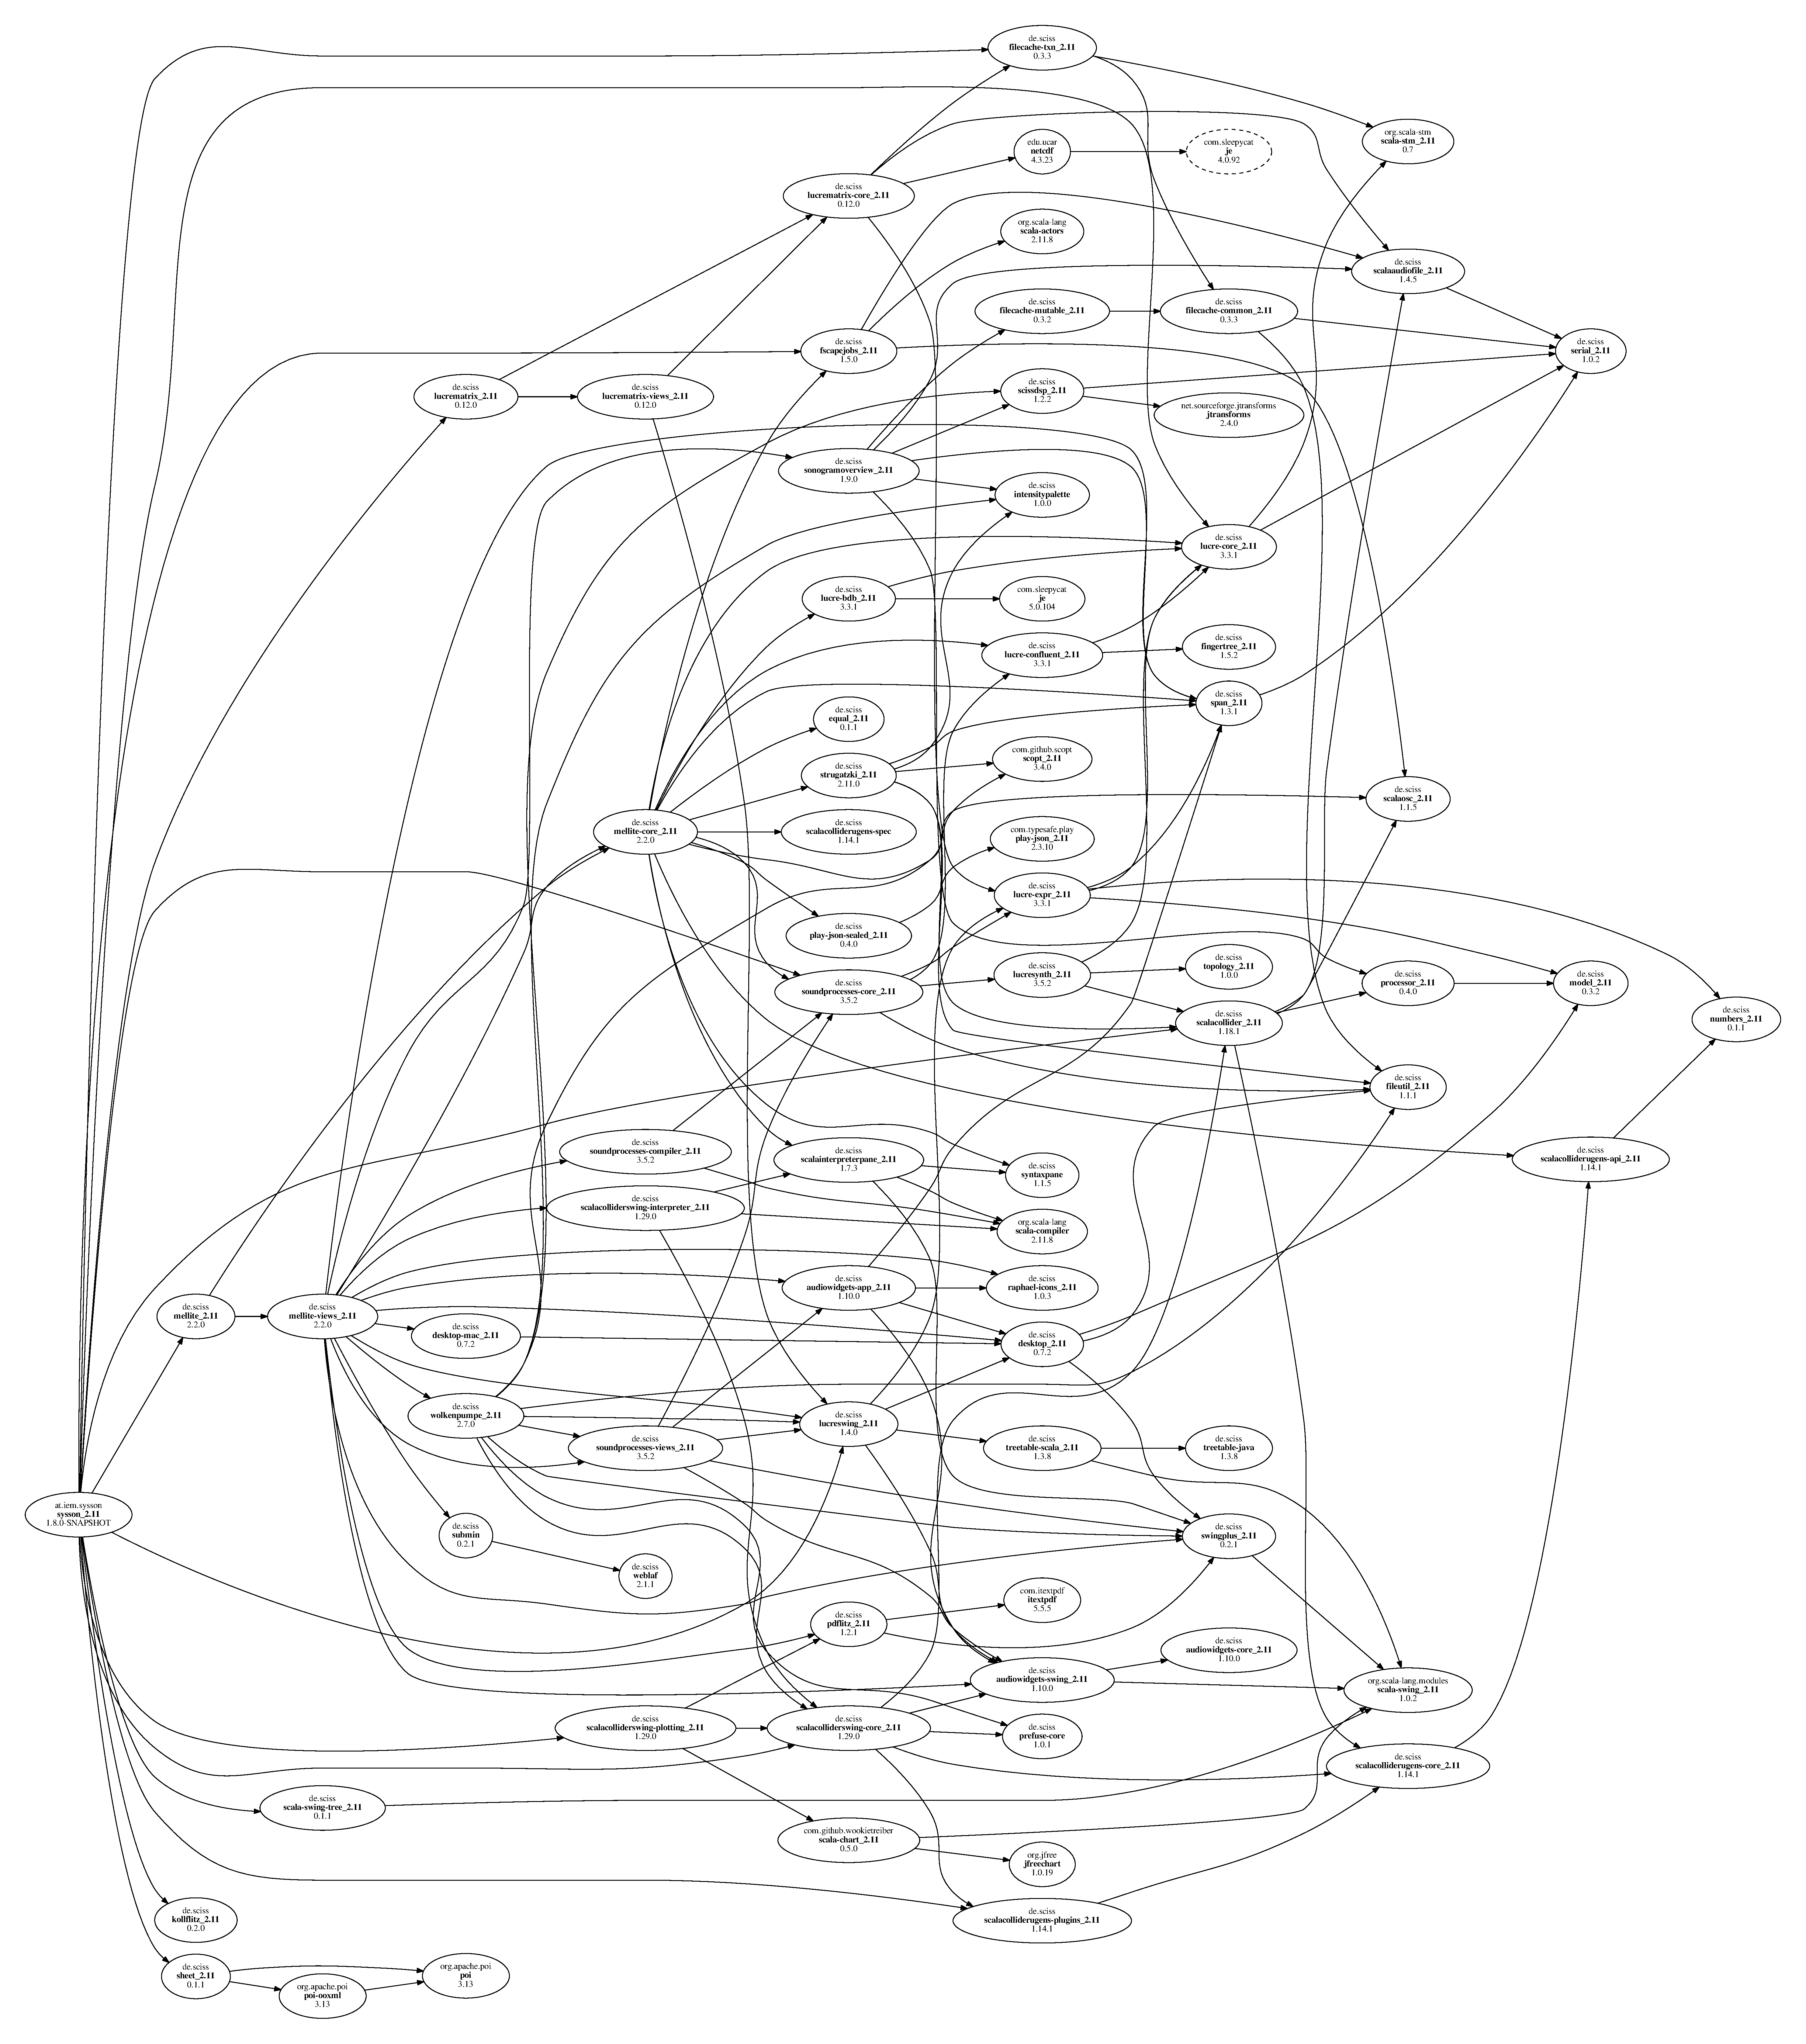
\includegraphics[width=\textwidth,trim=15mm 15mm 15mm 15mm]{figures/dependencies-compile.pdf}%
\caption{Module/library dependencies for SysSon version \syssonVersion{}}%
\label{fig:dependencies}%
\end{figure}

\subsection{Description of Modules}

We will now give a brief overview of the modules and libraries on which \sysson{} relies and which were shown in \figref{fig:dependencies}.

\paragraph{Mellite}

By far the strongest dependency is on the \software{Mellite} computer music environment. In fact, \sysson{} can be understood as a domain specific extension of \software{Mellite}, adding abstractions for sonification and matrix data, although the GUI is also slightly different.
%
Mellite is a graphical front end and application built on top of the \software{SoundProcesses} library. It introduces a tree based workspace structure with graphical views and editors for various objects.

\artefacts{} \verb!-core! contains objects in addition to \software{SoundProcesses}, such a color, the workspace and cursors abstractions, and a set of editing operations. \verb!-views! contains the graphical user interface, and undo-redo editing facilities.

\assessment{} The workspace abstraction should probably be moved directly into the \software{SoundProcesses} project, making the \verb!-core! artefact superfluous. It could be useful to define public API in a separate \verb!-api! artefact and create sub-modules for specific editors that do not necessarily have to be bundled in every application. An example is the \software{Wolkenpumpe} live improvisation tool that is currently a dependency of \verb!-views!.
A big challenge is the inter-linkage between visual representations and text-based editing. While the model-view approach already makes programmatic changes instantly visible across the UI, there is no global UI protocol through which the views ``know each other'' such that for example selecting one view implies a visual highlight on related views. Also because of the traditional windowing system, there are challenges in connecting objects (e.g. through ``cords'') across different windows. A radical revision of \software{Mellite} could focus on making text-editing a first class citizen, e.g. by allowing to activate a text-based view for every object on the UI. In terms of \sysson{}, an interesting model to look at might be the ``notebook'' approaches taken with software such as Jupyter.\footnote{\url{http://jupyter.org/}}

\paragraph{Lucre-Matrix}

Defined as a separate library, this module provides a matrix data abstraction, bridging \software{NetCDF} and the transactional-memory model defined by \software{Lucre} and underlying \software{SoundProcesses}. It makes it possible to build data-flow graphs, e.g. by applying a dimensional reduction operation to an input matrix, yielding a graph that constitutes a new compound matrix object.

\artefacts{} \verb!-core! contains the data structures, and a mechanism for caching matrix data in sound files (\sysson{}'s way of passing matrix data to \software{ScalaCollider}). \verb!-views! contains the graphical user interface element, noticeable as the matrix editor component in \sysson{}'s sonification editor.

\assessment{} The number of operations that can be performed on the matrices is quite small. It would also be worth exploring the possibilities of using a different matrix abstraction than the one of \software{NetCDF} as blue print, linking this library closer with standard ``data science'' frameworks. Another huge question arises from the way sonification models are built in \sysson{}. It appears that it may become much more important to be able to pre-process matrix data before they become part of the real-time sound synthesis. One way to conceive this is through additional ``graph elements'' in the sonification synthesis definition, i.e. as is done with elements such as \verb!Dim#values!. The down-side of this is that we risk duplicating the functionality on the ``Lucre side'' vs. the ``ScalaCollider side''. Therefore, the development of \software{Lucre-Matrix} very much depends on the evolution of the sonification model in \sysson{} and the way in which one will be able to represent ``sonification programs'', the way in which these programs can be ``co-edited'' with synthesis definitions.

\paragraph{Lucre}

The name \software{Lucre} serves as a placeholder for an approach to memory and data modelling based on software transactional memory (STM). \software{Lucre} defines an abstract system layer that usually occurs in objects as a type parameter \verb!S!, e.g. \verb!Sonification[S]!. At runtime, different systems can be initiated: an ephemeral pure in-memory system, a durable system where objects are automatically persisted to hard-disk, and a confluent system which extends the durable system with a version history of the modification of objects. This kind of temporal database approach has been developed extensively through my thesis \autocite{rutz2014tracing}, and forms the basis for \software{SoundProcesses}, \software{Mellite}, and \sysson{} respectively.

\artefacts{} There is currently no umbrella meta package. \verb!-core! is now a rather comprehensive artefact that includes four packages \verb!stm!, \verb!geom!, \verb!data!, \verb!event!. The reactive event propagation mechanism is now baked into the fundamental \verb!stm! package (this was not the case with older versions). This package defines the basic types \verb!Sys! (memory-model abstraction), \verb!Txn! (transaction), \verb!Cursor! (transaction initiator), \verb!Elem! (an element that publishes events and that can be copied), and \verb!Obj! (an element that in addition to \verb!Elem! has a unique identifier and an attribute map). Most data types in \sysson{} and and \software{SoundProcesses} inherit from \verb!Obj!. The \verb!event! package defines the infrastructure for event dispatch (publisher-subscriber mechanism). The \verb!data! package contains several data structures needed for the implementation of various systems, e.g. lists, trees, spatial search structures. The second artefact is \verb!-expr! that introduces reactive expressions, with implementations for primitive types such as strings, boolean values, integer and floating point numbers, time spans (a pair of 64-bit integers), collections---\verb!BiPin! for a ``flat'' sequence or breakpoint function, \verb!BiGroup! for a sequence with possibly overlapping elements---and \verb!Artifact! (file object). While in-memory and ephemeral-durable systems are defined in the base package, actual database back-ends are defined by \verb!-bdb! and \verb!-bdb6!, both using the \software{Berkeley DB Java Edition} (BDB DB JE), introducing the dependency on the GNU GPL. \verb!-bdb! uses version 5, compatible with the JVM version 6, and \verb!-bdb6! uses version 6, requiring JVM version 8. The \verb!-confluent! artefact implements the confluently-persistent (versioned) system.

\assessment{} Changes in \software{Lucre} fundamentally affect all parts of \sysson{}, as it is a deep dependency that is used by \software{SoundProcesses}, \software{Mellite}, \software{Lucre-Matrix} and others. The current version is stable and reliable but has a number of shortcomings: On the programming level, the syntactic overhead of carrying around system type parameter \verb!S <: Sys[S]]! as well as transaction context method argument \verb!implicit tx: S#Tx! is high, making it a rather bad fit for a light-weight domain specific language to define snippets in \software{Mellite} or \sysson{}. In the medium term future, this might be alleviated by the next generation Scala language (Dotty research project), where on the one hand type projections are seriously constrained, probably making it necessary to redefine the way system abstraction is visible in \software{Lucre}, but on the other hand also allowing to ``hide'' type parameters as type members and implicit arguments as implicit capabilities of a function's return type. However, this is a perspective of several years into the future, so in the shorter term, probably the most convincing solution is to add a separate DSL layer where transactional semantics are injected into the interpreter's code execution. Another question concerns the cost of \verb!Obj! instances. In previous versions we distinguished between expressions and these objects, making it for example possible to have cheap constant values. Constants appear very frequent, for example if one edits a numeric value in \sysson{} through a slider, many new objects have to be created (and persisted to the database) for each intermediary state in the dragging operation. With \verb!Obj! being basically the atoms for most operations, this means that now we have to allocate a lot of throw-away object identifiers and the space usage in the database is much higher than with the old ``simple'' constants, where only the containing \verb!S#Var! variable (mutable placeholder) was requiring a one-time allocation. It is thus desirable to rethink this atomicity and try to combine the simplicity of one layer \verb!Obj!-everywhere with the performance of having cheap constants. Somehow related to this is the lack of any sort of automatic garbage collection for transitory values. If we had a reference counting ability, we could evict objects from the database once they are not reachable any longer, or those transitorily produced during a transaction without having an actual linkage to the workspace at the commit-time of the transaction. A reference tracking could also help with automatically detecting ``bottom-up'' dependencies between objects in the GUI. Furthermore, we need to assess the necessity for the full confluent persistence in versioning---while theoretically elegant, we cannot abstract over the meld operation in the system layer, because there is no equivalent for ephemeral systems. Therefore, we are forced to introduce a object-copying mechanism agnostic of the system capabilities. Also, confluent meld could become expensive if used excessively, as the version paths grow linearly with the levels of meld. It might thus be more pragmatic to simplify the versioning system by moving to the less powerful partial persistence and improving on the definition of object-copying. Object-copying could also preserve information about the source object from which a copy was made, as this information is currently lost and thus undermines the effort to version objects. Another problem is the size of transactions. Transactions can become quite large which poses a problem for the database commit phase, as ACID requires that we wait for the durability guarantee at the end of each transaction. There is a ticket\footnote{\url{https://github.com/Sciss/Lucre/issues/6}} to evaluate other database back-ends, something that will also interact with the \software{Serial} module. It seems that especially in concurrent situations with conflicting transactions, we face performance problems or even impasses where the database times out. Going away from STM as the memory model would however require an entire new architecture, and so far STM has proven a very robust approach, so it is probably advisable to stay with it for the time being, instead evaluating strategies to undo the bottle-necks with concurrent transactions.

So far we have used BDB DB JE 5 to allow \sysson{} to run on legacy computers with Java 6, such as Mac OS X 10.6. The next version of \sysson{} can probably drop that constraint and require presence of Java 8 and thus the newer database version.

\paragraph{Scala-STM}

The reference implementation for software transactional memory in Scala. 

\assessment{} This library is quite stable, error free, and fast. The only bottle neck is using a decider-hook when coupling to a database transaction that must be completed with the \software{Scala-STM} transaction. For performance reasons, implicit transaction values have to be carried around when defining a transactional API, although the library also allows the lookup of transactions from a thread-local variable and the automatic coalescence of transactions if one unknowingly starts a new \verb!atomic {}! block. Care has to be taken in nested functions to prevent catching a stale implicit transaction context from an other function. From experience, the best solution to this problem is to move transactional methods all to the top-level of an object and avoid nesting them.

\paragraph{Lucre-Swing}

Published as a separate library, this module provides a set of simple widgets that can interface with expressions and other data structures from the \software{Lucre} project.

\paragraph{Serial}

This module defines a small serialization layer used by \software{Lucre} and other libraries.

\assessment{} The module is optimised for speed and size, making serialization quite efficient. However, a current drawback is vulnerability to schema evolution. Serialised objects simply become unreadable if the schema is altered without any precautions in place that can parse older versions. In many cases it may simply not be possible to parse older versions, and in those cases it would be required to entirely ``upgrade'' an objects, for example allocating additional objects. While such upgrades are currently not foreseen, there are also made nearly impossible by the fact that the same entity might be written multiple times in the database. If every \verb!Obj! with an identifier \verb!S#ID! would be written as a small reference to one and the same location in the database, perhaps upgrading schemas would become feasible. For robustness, it would also be very helpful if an automatic export to other formats such as JSON would be available. This would require the serialisation API to change, for example including field names. Another current limitation is the prohibition of reference cycles within the same serialisation, something that can currently be worked around by the indirection of a \verb!S#Var!. Finally, one must currently write serialisers by hand which from our experience is \emph{very} prone to errors, and also clutters the source code unnecessarily. After deciding on an updated API, it might thus be advisable to look into macro-based synthesis of serialisers.

\paragraph{SoundProcesses}

Sound synthesis abstractions are provided by the \software{SoundProcesses} module which can be understood as bridge between lower-level sound synthesis library \software{ScalaCollider} and the \software{Lucre} memory model. \software{SoundProcesses} defines an abstraction \verb!Proc! that encapsulates a sound synthesis function with a dictionary of controllers and resources. It makes it safe to connect and alter sound processes transactionally, automatically providing correct node topology, resource management, and real-time dispatch. A notion of aural-views is introduced, translating the MVC concept from the visual domain to sound. \software{SoundProcesses} is described in detail in my thesis, as well as in several conference papers (e.g. \cite{rutz2014sound}).

\artefacts{} There is currently no umbrella meta package. The \verb!-synth! sub-module (full artefact-identifier \verb!lucresynth!) is a transactional layer on top of \software{ScalaCollider}. For every imperative API in \software{ScalaCollider} we have a transaction-safe equivalent here, e.g. playing a \verb!Synth!, allocating and filling buffers, etc. A new \software{Lucre} system layer is defined that handles OSC messages to the \software{SuperCollider} server. The \verb!-core! sub-module then is the meat of \software{SoundProcesses}. It defines the \verb!Proc! object, several general purpose objects such as folders (reactive lists), graphemes (breakpoint functions), actions (functions triggered for example by a \verb!Proc!), fade-specifications, and curvatures. Furthermore, an offline and real-time scheduler and transport mechanism, and a timeline object. The \verb!AuralView! type introduces the model-view separation on the audio level. The \verb!graph! sub-package defines a number of pseudo-UGens necessary for accessing the attributes associated with a \verb!Proc! (controllers, buffers, etc.). The \verb!-compiler! sub-module defines a small abstraction for an embedded Scala compiler, which in turn is provided by the \software{Scala-Compiler} dependency. This compiler is used in the user-interface for ad-hoc compilation of source code fragments. The \verb!-views! sub-module defines a number of specific widgets, such as a volume meter, time display and transport control buttons.

\assessment{} The automatic resource management and OSC timing can be quite intricate, and as a result, some of the code base internals are quite complex and could benefit from simplification and modularisation. The aural view implementations also become quite complicated because of the necessity to update actual real-time views according to the appearance and disappearance of model dependencies (e.g. when a missing buffer association is added or removed). This is also in part due to the way synth graphs are assembled, currently requiring control exceptions to be thrown with partially built synth graphs to be properly maintained and incrementally updated. Composition poses another difficulty. For example, in \sysson{}, the \verb!Sonification! object encapsulates a \verb!Proc!, but it must make its own attribute map available for the aural-view building, requiring a variant of the aural view that relies on the internal implementation of the aural view of \verb!Proc!. A general drawback is that we cannot directly monitor ``capabilities'' of a sound process introduced by specific (pseudo-)UGens. For example, in \sysson{} we must scan the synth graph for objects that have consequences on the sonification editor, such as matrix and dimension variables appearing or disappearing. Providing for better ``functionally reactive'' filtering of the synth graph could improve the situation. In general, the monolithic shape of the synth graph could be seen as problematic. For example, in the \sysson{} ``Science by Ear 3'' workshop, some participants familiar with \software{SuperCollider} felt constrained by the lack of support for small functions, patterns and routines, and so on. Chaining this functionality together with imperative \verb!Action! objects seems rather inelegant. % Another problem again are the missing ``bottom up'' references.
Currently, there are no guarantees with respect to the precise OSC bundle scheduling. The scheduler is based on a client CPU timer, bundles are properly constructed with respect to transactional atomicity, but it is not possible to ensure that for example an event happening exactly one second after another will execute on the server after the corresponding number of sample frames. This is mainly a problem for timeline composition and less so for sonification, but it will become a problem if we add more client side timing, such as routines, to sonification. Another timing issue occurs with preparation times. There is a rudimentary mechanism in place to allow for a \verb!Proc! to prepare resources asynchronously---e.g. loading a very large buffer---and this is also used by \sysson{} for caching matrix data. But again, for sequencing objects, we need to add information about expected latencies or at least allow for the customisation of the preparation pre-delay. In terms of the GUI, it may seem counter-intuitive that one has to wait sometimes quite long for data to be prepared after pressing the play button. We need at least a clear visual indicator here.

\paragraph{ScalaCollider}

\software{ScalaCollider} is a client for the \software{SuperCollider} server, driving its real-time sound synthesis engine. It is stable and quite feature complete and should allow anyone familiar with \software{SuperCollider} to be able to quickly write sound synthesis definitions, even if the implementing language---Scala---is a different one.

\artefacts{} The unit generators (UGens) and their basic API are separately defined in the \verb!-ugens! projects with its own sub-modules \verb!-api! (abstract UGen API only), \verb!-core! (standard UGens bundled with \software{SuperCollider}), \verb!-plugins! (incomplete set of third-party UGens), and \verb!-spec! (XML meta-data with UGen descriptions). The main project consists of one artefact only. It adds an actual UGen graph builder and server object, bus abstractions, an imperative layer for running synthesis processes. Another project \verb!-swing! introduces an integrated development environment (IDE), a desktop application a bit simpler than the original \software{SuperCollider IDE}. It is split into the sub-modules \verb!-core! which contains individual widgets (e.g. node tree visualisation, server status panel), \verb!-interpreter! which connects to the Scala interpreter, \verb!-plotting! which adds simple plot command based on \software{Scala-Chart}, and \verb!-app! which bundles all together as a standalone desktop application.

\assessment{} \software{ScalaCollider} is a more or less ``finished'' product, the architecture is simple and works as expected. It currently does not include any abstractions for client-side scheduling, such a tasks or routines, but this is probably an advantage as we could in any case not use them directly but would have to translate them to the transactional \software{Lucre} model. The IDE uses the \software{Docking-Frames} window docking library which seems good enough for the task. While the \software{WebLaF} introduces its own docking mechanism in the upcoming release, sticking to \software{Docking-Frames} might be advisable also for \software{Mellite} and \sysson{}, because it is independent of the look-and-feel used and does not imposes the GNU GPL 3 license. Widget and plotting functionality could be extended and should be better integrated with or made available in \sysson{} whose interpreter mode is currently neglected.

\paragraph{Desktop}

This artefact provides simple abstractions for desktop application, based on Swing, such as the notion of a document in a multi-document application (MDA), or user preferences storage. For windowing, it has the notion of a shared menu-bar, and an abstraction for windows that can be realised both as standalone windows or windows internal to one screen-filling containing frame.

\artefacts{} Apart from \verb!-core!, there are sub-modules for the different operating systems, e.g. \verb!-mac! and \verb!-linux!. There are platform independent operations such as showing a file in the desktop manager, that are implemented differently per platform. 

\assessment{} The library is quite simple. Especially the menu-bar management comes still with some OS X baggage, where one shared menu-bar across windows is standard. It would also be helpful to directly incorporate some docking framework.

\paragraph{Audio-Widgets}

A library with audio-related widgets for graphical user interfaces, such as volume meters or transport controls.

\artefacts{} The \verb!-core! module contains individual widgets directly implemented on top of \software{Java-Swing}, while the \verb!-swing! module wraps them for \software{Scala-Swing}. The \verb!-app! module is very small and adds an abstraction for timeline based canvases.

\paragraph{Swing-Plus}

This library extends \software{Scala-Swing} with a few missing widgets.

\paragraph{Scala-Swing}

This library wraps the \software{Java-Swing} cross platform widget toolkit in an API that is more elegant to use from Scala. For example, event handling is greatly simplified.

\paragraph{Scala-Swing-Tree}

An improved model/view widget combination for tree based data structures.

\paragraph{Tree-Table}

A custom Swing widget combining a tree-like structure with a table (multiple columns) view. Artefacts exist for Java and a Scala wrapper.

\paragraph{Scala-Chart}

A simple Scala wrapper and DSL for accessing the \software{JFreeChart} charting library. \software{JFreeChart} is the most mature and widely used Java charting/plotting library based on Swing.

\paragraph{Sonogram-Overview}

A constant-Q based transform library for producing sonograms from sound files. This is used by Mellite editors to view sound files or sound regions as sonograms.

\assessment{} The library implements a pyramidial decimation approach to creating multi-resolution images. The sonograms are written to cache files formally as audio files. There is currently no mechanism in place manage ad-hoc changes in resolution, such as zooming in or out of a sonogram that triggers more coarse or fine recalculations. There is a graphical glitch in region display where block boundaries are seen as vertical stripes. The algorithm is quite expensive, so calculating many sonograms for many sound files takes long time and occupies a lot of hard-disk space.

\paragraph{Intensity-Palette}

A psycho-optically optimised colour palette, adapted from the \software{Sonasound} software. Used as the default scheme for rendering sonograms.

\paragraph{Sciss-DSP}

A DSP library containing a few basic algorithms such as FFT, Wavelet decimation, band-limited resampling, FIR filters and window functions. FFT is now based on the \software{JTransforms} library.

\paragraph{JTransforms}

A fast Java FFT library with single and double precision, real and complex, and one- or two-dimensional support.

\assessment{} The library is quite fast. By default parallelism is activated, but it can be configured to run single-threaded if needed.

\paragraph{File-Cache}

A simple library for managing hard-disk cache of expensive calculations. This is for example used for sonogram caching and for matrix-to-audio-file translation cache in \sysson{}. 

\paragraph{File-Util}

A simply utility library for constructing files and paths.

\paragraph{Scala-Interpreter-Pane}

A Swing widget built around the Scala compiler/interpreter and a text editor with syntax highlight.

\assessment{} The interpreter is a thin layer on top of Scala's own \verb!IMain! interpreter structure. Similar to the \software{SuperCollider IDE}, pressing control and return executes the selected text or the current line. An interesting alternative could be that executed source code is appended to a sort of protocol so that it becomes easier to reproduce a REPL session. This might be similar to how the ``notebook'' approaches of IPython/Jupyter work. Another model currently seen is the ``worksheet'', where a ``hot'' interpreter continuously evaluates the entire source code and prints the results of each statement on the right-hand side of the code. With respect to the text editor, the code highlight is rather simple and based on the \software{Syntax-Pane} artefact, which is just a lexer without further code analysis. There are more advanced systems such as \software{ENSIME}\footnote{\url{http://ensime.github.io/}} that improve on code completion, look-up, type checking and inspections, and so forth. There are also improved REPLs such as \software{Ammonite}\footnote{\url{http://www.lihaoyi.com/Ammonite/}} that claim better code completion. On the other hand it would be interesting to explore possibilities of representing placeholders for objects in the GUI in the text editor. Custom widgets such as live sliders are for example implemented in \software{Field}\footnote{\url{http://openendedgroup.com/field/}} \autocite{downie2008field}, and there are vocal proponents of more visually interactive systems such as Bret Victor\footnote{See for example \url{http://worrydream.com/\#!/TheFutureOfProgramming} and \url{http://worrydream.com/\#!/MediaForThinkingTheUnthinkable}; 
also the work of Sean McDirmid on ``live programming'' \autocite{mcdirmid2013usable}.}.

%\paragraph{Scala-Compiler}
%
%\paragraph{Syntax-Pane}

\paragraph{Sheet}

This is a simple library for reading spread sheet data from Excel files, based on the Apache POI library. It is used as an import function in \sysson{}.

\paragraph{NetCDF}

The \software{NetCDF} is written by UCAR and was used in \sysson{} because all the climatology data was in \verb!.nc! NetCDF format. The library contains its own matrix and array data types.

\assessment{} The file access is not thread-safe, so one has to throw a \verb!synchronized {}! block at it. We currently only use synchronous reading, but it might be the case that asynchronous I/O is also supported (to be evaluated).

\paragraph{Submin}

A combination of light (dark text on bright background) and dark (light text on dark background) ``skins'' for the Web-look-and-feel, the cross platform Swing-based look used in \software{Mellite} and \sysson{}.

\assessment{} The underlying \software{Web-Look-And-Feel} is currently under development for a release version 1.29. The GNU GPL 3 licenses is unfortunate and we therefore strive to avoid any hard dependencies on this look and feel. All GUI in \software{Mellite} and \sysson{} is written agnotic to the look-and-feel selected. Therefore, depending on Web-LaF's docking framework would be a serious decision. The LaF is also quite large and not extremely fast in comparison to other Swing LaFs. There were a few issues with keyboard shortcuts on OS X that are probably resolved by now. On the up-side, it is probably one of the best looking LaFs available, with the light scheme directly taken from Web-LaF, and the dark scheme designed by me but closely based on the light scheme. \sysson{} is not yet fully tested with the dark scheme and might need some customisation to support both light and dark scheme.

\paragraph{Raphael-Icons}

The icon set used by \software{Mellite} and \sysson{} is mostly based on \software{Raphael.js}, and the original SVG graphics have been converted to a simple library dependency.

\assessment{} Translating the SVG to code may have actually been a bad idea, as the library can become quite large. Perhaps a better approach is a fast SVG path parser and preservation of the SVG path strings.

\paragraph{Prefuse}

\software{Prefuse} is used to render dynamic graphs in the \software{Wolkenpumpe} live improvisation interface, but also other widgets such as \software{ScalaCollider-Swing}'s node tree view.

\paragraph{Wolkenpumpe}

Bundled with \software{Mellite} but should probably be optional. A live improvisation interface, otherwise not used in \sysson{}.

\paragraph{Strugatzki}

Bundled with \software{Mellite} but should probably be optional. A basic music-information-retrieval kit, based on \software{ScalaCollider}.

\paragraph{FScape-Jobs}

Bundled with \software{Mellite} but should probably be optional. A simple OSC client library to issue DSP jobs through \software{FScape}. We are currently rewriting \software{FScape} based on a finer UGen granularity, Scala, and Akka-Stream. This new version 2 will make \software{FScape-Jobs} eventually obsolete.

\paragraph{Processor}

An interface for defining asynchronous offline rendering jobs, extending Scala's \verb!Future! with the ability to cancel the job and to monitor progress.

\paragraph{Model}

A simple library for publisher-subscriber functionality.

\paragraph{Finger-Tree}

A versatile functional data structure that is used here mainly as an immutable data structure for sorting intervals.

\paragraph{Topology}

A data structure for maintaining an online directed graph. When edges are inserted, the caller gets information on how vertices have to been moved to correctly preserve a linear order. Used for example by \software{SoundProcesses} to automatically reshuffle \verb!Proc! instances a they are interconnected.

\paragraph{Span}

A pair of start and stop sample frames defines a time span in \software{SoundProcesses} and \sysson{}.

\paragraph{Scala-OSC}

The Open Sound Control library used by \software{ScalaCollider}.

\paragraph{Equal}

A simple library allowing for more type-safe comparisons of values through the \verb!===! (triple-equals) and \verb$!==$ operators.

\paragraph{Play-JSON-Sealed}

An extension of the JSON library that is part of the \software{Play} framework, allowing the automatic macro based construction of serialisation code for sealed type hierarchies (algebraic data types).

\assessment{} Scala does not have a standard JSON library (its standard library does contain some rudimentary JSON functions but they are generally considered inferior to any other library), and as a consequence there are now dozens of alternatives available. We found Play JSON to be fairly simple and straight forward, with its macro based serialisation generation freeing one from writing serialisers by hand. It might still be worth to evaluate other JSON libraries.

\paragraph{Numbers}

A library that enriches number types with operator often known from \software{SuperCollider} and \software{ScalaCollider}. For example we can write \verb!2.0.sqrt! or \verb!7.nextPowerOfTwo!.

\paragraph{PDFlitz}

A thin wrapper around \software{iText PDF}, allowing especially the export of any Swing or Java2D component as a PDF file. Enforces a GPL v3+ license.

\paragraph{Koll-Flitz}

A library that enriches collection types with useful operators such as iterating or mapping over pairwise groups.

\printbibliography

\end{document}